\documentclass[11pt]{article}
\usepackage[utf8]{inputenc}
\usepackage{geometry}
 \geometry{
 a4paper,
 total={170mm,257mm},
 left=20mm,
 top=20mm,
 }
 \usepackage{graphicx}
 \usepackage{titling}
 \usepackage{amsmath}
 
\usepackage{subcaption}

\usepackage[backend=bibtex,style=ieee]{biblatex}
\bibliography{bibliography}

\usepackage{mathtools}
\DeclarePairedDelimiter\ceil{\lceil}{\rceil}
\DeclarePairedDelimiter\floor{\lfloor}{\rfloor}

 \title{An approach to parallel Matrix Multiplication using MPI}
\author{Riccardo Zuech}
\date{July 2024}
 
 \usepackage{fancyhdr}
\fancypagestyle{plain}{%  the preset of fancyhdr 
    \fancyhf{} % clear all header and footer fields
    \fancyfoot[L]{\thedate}
    \fancyfoot[R]{Repository: https://github.com/ZuechR/ParallelMM}
    \fancyhead[L]{Parallel Computing Laboratory Project}
    \fancyhead[R]{\theauthor}
}
\makeatletter
\def\@maketitle{%
  \newpage
  \null
  \vskip 1em%
  \begin{center}%
  \let \footnote \thanks
    {\LARGE \@title \par}%
    \vskip 1em%
    %{\large \@date}%
  \end{center}%
  \par
  \vskip 1em}
\makeatother

\usepackage{lipsum}  
\usepackage{cmbright}

\begin{document}

\maketitle

{
\centering
\begin{tabular}{@{}ll}
    Student & \theauthor:  2128872\\
    Teachers& Gianfranco Bilardi\\
 &Paolo Emilio Mazzon\\\end{tabular}
\par}

\section{Problem Definition}

Matrix multiplication is a fundamental operation appearing in many problems across different fields, thus finding ways to speed-up its execution is a topic of great interest.

The matrix multiplication problem is usually defined as follows:

Given a matrix $\textbf{A}$ of size $MxN$ and a matrix $\textbf{B}$ of size $NxO$
\[ \textbf{A} = \begin{pmatrix}
    a_{0, 0} & a_{0, 1} & \cdots & a_{0, N-1} \\
    a_{1, 0} & a_{1, 1} & \cdots & a_{1, N-1} \\
    \vdots  & \vdots  & \ddots & \vdots  \\
    a_{M-1, 0} & a_{M-1, 1} & \cdots & a_{M-1, N-1} 
\end{pmatrix} \quad\quad \textbf{B} =
\begin{pmatrix}
    b_{0, 0} & b_{0, 1} & \cdots & b_{0, O-1} \\
    b_{1, 0} & b_{1, 1} & \cdots & b_{2, O-1} \\
    \vdots  & \vdots  & \ddots & \vdots  \\
    b_{N-1, 0} & b_{N-1, 1} & \cdots & b_{N-1, O-1} 
\end{pmatrix} \]
let $\textbf{C} = \textbf{AB}$ be the matrix of size $MxO$:
\[ \textbf{C} = \begin{pmatrix}
    c_{0, 0} & c_{0, 1} & \cdots & c_{0, O-1} \\
    c_{1, 0} & c_{1, 1} & \cdots & c_{1, O-1} \\
    \vdots  & \vdots  & \ddots & \vdots  \\
    c_{M-1, 0} & c_{M-1, 1} & \cdots & c_{M-1, O-1} 
\end{pmatrix} \quad\quad \text{such that:  }
c_{i, j} = \sum_{k=0}^{N - 1} a_{i, k}b_{k, j} \]

\subsection{Sequential algorithm}
As the sequential algorithm, we adopted the straightforward algorithm descending from the above definition (with the addition of a few useful tricks).
Essentially, our algorithm performs the computation of $\textbf{C}$ element per element, in row-major order, by the above formula.

Additionally, our implementation also includes the use of two techniques:
\begin{itemize}
    \item All the matrixes are stored as arrays, in particular as sequences of rows.
    \item The algorithm is adapted to multiply matrix $\textbf{A}$ with the transpose $\textbf{B}^\top$ of matrix $\textbf{B}$.
\end{itemize}
The combination of these techniques is used in order to take advantage of the well-known cache mechanisms to allow for an overall faster execution compared to a matrix-centered approach.
For the sake of brevity, the technical details of the sequential algorithm implementation are omitted from this report and can be found in the repository.

The choice of this algorithm is motivated by the following points:
\begin{itemize}
    \item We wanted to solve the general case for any value of $M,N,O \in {\rm I\!R}^+$ such that $M,N,O > 0$. Faster algorithms exist for special cases, but we preferred to keep our study on the most generalizable case possible.
    \item The general algorithm can easily and straightforwardly be reused in the parallelized version, as we will see later.
\end{itemize}

On a final note, it's easy to see that our algorithm always requires time $T_{\text{seq}} = \Theta(M\cdot N \cdot O)$.
\section{Parallelization Approach}

Our approach to parallelization derives from the observation that, given as "known" the matrix $\textbf{B}$, the rows of $\textbf{C}$ can be computed independently of each other on the base of the corresponding rows of $\textbf{A}$.

Let us have $P$ processors under the SPMD paradigm, then our solution is based on defining a master process (the one with rank $0$) whose role is to:
\begin{enumerate}
    \item Initialize the values of matrix $\textbf{A}$ and $\textbf{B}$, then converting $\textbf{B}$ into $\textbf{B}^\top$.
    \item Broadcast $\textbf{B}^\top$ to every other process using \texttt{MPI\_Bcast}.
    \item Evenly distribute sets of adjacent rows of $\textbf{A}$ to each process (the master itself included) using \texttt{MPI\_Scatterv}. \\ Note that \texttt{MPI\_Scatterv} is used over \texttt{MPI\_Scatter} since we may have a number $M$ of rows that is not divisible by $P$; in this case we assign $\floor*{M/P} + 1$ rows to the first $M \textit{ mod } P$ processes, and then $\floor*{M/P}$ to the remaining ones.
    \item Store the final output matrix $\textbf{C}$.
\end{enumerate}

Let us refer to $\textbf{A}_p$ as the set of adjacent rows of $\textbf{A}$ assigned to the process $p$, then we also define $\textbf{C}_p$ as the set of adjacent rows of $\textbf{C}$ produced by the process $p$ by calling the sequential algorithm for matrix multiplication on $\textbf{A}_p$ and $\textbf{B}^\top$.

Then, as the final step, we use \texttt{MPI\_Gatherv} to gather the $\textbf{C}_p$ produced by each process into $\textbf{C}$ in the master process, in the correct order. We use \texttt{MPI\_Gatherv} over \texttt{MPI\_Gather} by the same argument discussed for \texttt{MPI\_Scatterv}.

For the sake of brevity, we omit the technical discussion about the specifics of the implementation, which can be found in the repository.

\subsection{Performance gain of parallelization}\label{ssec:pperform}

It is straightforward to see that the execution time of our parallelized algorithm takes time $T_{\text{parallel}} = T_{\text{comp}} + T_{\text{comm}}$, where $T_{\text{comp}}$ is the time that the master process needs to compute $\textbf{C}_0$ (its portion of $\textbf{C}$) and $T_{\text{comm}}$ is the time spent for communication from the "point of view" of the master.

On a theoretical level, we have $T_{\text{comp}}^p = \Theta(M/P \cdot N \cdot O)$ for any process $p$, since each process either receives $\floor*{M/P}$ or $\floor*{M/P} + 1$ rows of $\textbf{A}$. Essentially, excluding the communication time, the parallelization of the sequential algorithm allows achieving a theoretical speed-up factor of $P$.

The analysis of the communication time instead is not easy and cannot be generalized to a theoretical bound, since it depends on the specific characteristics of the network used, the positions of the processors assigned to our job, the load of the whole system at the time and so on.

However, taking the time from the broadcasting of \textbf{B} to the gathering of \textbf{C} in the master process, and subtracting $T_{\text{comp}}^0$, we get $T_{\text{comm}}$ for that specific execution of the algorithm. It is interesting to point out that the communication time obtained this way provides a lower bound on worst-case true communication time on the underlying system by the existential argument.
\section{Experimental results}

\begin{table}[!ht]
    \centering
    \caption{Execution time of the sequential and parallel algorithms for different matrices sizes and number of processors $P$.}
    \begin{subtable}{.45\linewidth}
        \centering
        \caption{$\textbf{A}$ \& $\textbf{B}$ of size 512x512}
        \begin{tabular}{r|r|r}
            \textbf{P} & \textbf{T\_comm} & \textbf{T\_comp} \\ \hline
            \textbf{Seq} & 0 & 50.003 \\ \hline
            \textbf{1} & 1.674681 & 50.461275 \\ \hline
            \textbf{2} & 11.206590 & 25.225144 \\ \hline
            \textbf{4} & 16.922512 & 12.566901 \\ \hline
            \textbf{8} & 32.924253 & 6.344639 \\ \hline
            \textbf{16} & 148.222790 & 3.223668 \\ \hline
            \textbf{32} & 174.169211 & 1.710644 \\ 
        \end{tabular}
    \end{subtable}
    \begin{subtable}{.45\linewidth}
        \centering
        \caption{$\textbf{A}$ \& $\textbf{B}$ of size 1024x1024}
        \begin{tabular}{r|r|r}
            \textbf{P} & \textbf{T\_comm} & \textbf{T\_comp} \\ \hline
            \textbf{Seq} & 0 & 388.730 \\ \hline
            \textbf{1} & 4.030184 & 387.597033 \\ \hline
            \textbf{2} & 19.815538 & 195.856201 \\ \hline
            \textbf{4} & 32.914310 & 101.572801 \\ \hline
            \textbf{8} & 51.866337 & 60.452539 \\ \hline
            \textbf{16} & 199.891284 & 38.215937 \\ \hline
            \textbf{32} & 300.292535 & 12.898068 \\ 
        \end{tabular}
    
    \end{subtable}
    \begin{subtable}{.45\linewidth}
        \centering
        \caption{$\textbf{A}$ \& $\textbf{B}$ of size 2048x2048}
        \begin{tabular}{r|r|r}
            \textbf{P} & \textbf{T\_comm} & \textbf{T\_comp} \\ \hline
            \textbf{Seq} & 0 & 3768.356 \\ \hline
            \textbf{1} & 13.511889 & 3819.322627 \\ \hline
            \textbf{2} & 70.904731 & 2941.665213 \\ \hline
            \textbf{4} & 67.533221 & 1335.798456 \\ \hline
            \textbf{8} & 138.074651 & 707.863888 \\ \hline
            \textbf{16} & 123.805203 & 338.441502 \\ \hline
            \textbf{32} & 275.721030 & 139.956284 \\ 
        \end{tabular}
    
    \end{subtable}
    \begin{subtable}{.45\linewidth}
        \centering
        \caption{$\textbf{A}$ \& $\textbf{B}$ of size 4096x4096}
        \begin{tabular}{r|r|r}
            \textbf{P} & \textbf{T\_comm} & \textbf{T\_comp} \\ \hline
            \textbf{Seq} & 0 & 50192.182 \\ \hline
            \textbf{1} & 54.562895 & 51104.039326 \\ \hline
            \textbf{2} & 114.210136 & 25177.496365 \\ \hline
            \textbf{4} & 251.198126 & 11896.659449 \\ \hline
            \textbf{8} & 406.719612 & 6237.871031 \\ \hline
            \textbf{16} & 244.012867 & 3085.359583 \\ \hline
            \textbf{32} & 474.394116 & 1654.710260 \\ 
        \end{tabular}
    
    \end{subtable}
    
    \label{tab:results}
\end{table}

In the experimental phase, we utilized the CAPRI \cite{1} platform to run the sequential and parallel algorithms through the SLURM scheduler. In particular, the C code has been compiled using the \textit{-O3} flag for both algorithms and compilers \textit{mpicc} and \textit{gcc} for the parallel and sequential algorithm respectively.

For simplicity of analysis, we decided to run the algorithms with square matrices of size power of 2 on powers of 2 of processors $P$; in particular the matrices are arbitrarily initialized with integers chosen uniformly at random in the range $[-99, 99]$, since the focus of this work is on the algorithms implementation and analysis.

Additionally, for each combination of sizes and number of processors, we run the algorithms a total of 5 times and take the averages as the final data. Table \ref{tab:results} reports the average results of our runs; additionally, the data for each run is also available in the repository.

As an important note, all the measurements were done on the minimal set of relevant operations, this means that from the computed times we excluded all the initialization operations, e.g. the allocation of space for $\textbf{A}$,$\textbf{B}$ and $\textbf{C}$, as well as the construction of the auxiliary data structures.

\subsection{Time performance}

Let us now consider the comparison between time performance of the sequential algorithm and the parallel algorithm, as presented in Figure \ref{fig:time_size}.

\begin{figure}[hb!]
    \centering
    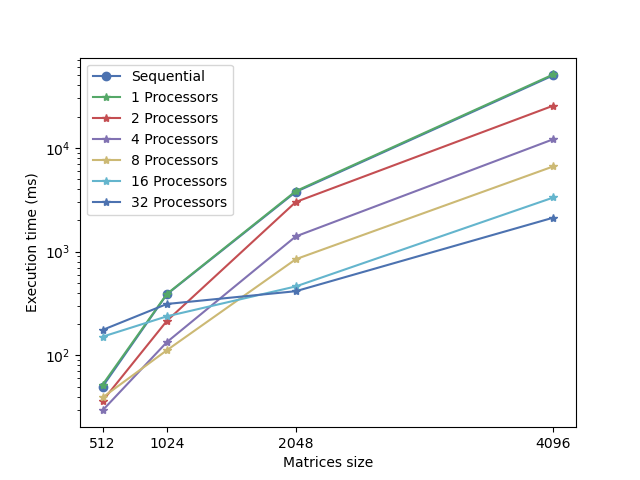
\includegraphics[width=0.8\linewidth]{figures/time_size.png}
    \caption{Time performance over matrix sizes of the sequential algorithm and parallel algorithm on a different number $P$ of processors.}
    \label{fig:time_size}
\end{figure}

As expected, we observe the well-known trade-off between computation time and communication time for higher numbers of processors characteristic to parallel algorithms: for small matrices, the communication requirements overshadow by a significant margin the gain in computation time, while for bigger matrices the distribution of the computation across many processors enables a big enough gain to greatly compensate for any time spent communicating. 
For example, from Table \ref{tab:results} we can see that for $P \ge 16$ and $M=N=O < 2048$ the communication time required to spread and gather data across this many processors takes a temporal toll that is greatly bigger than the computation time of the distributed matrix multiplication.

\begin{figure}[hb!]
    \centering
    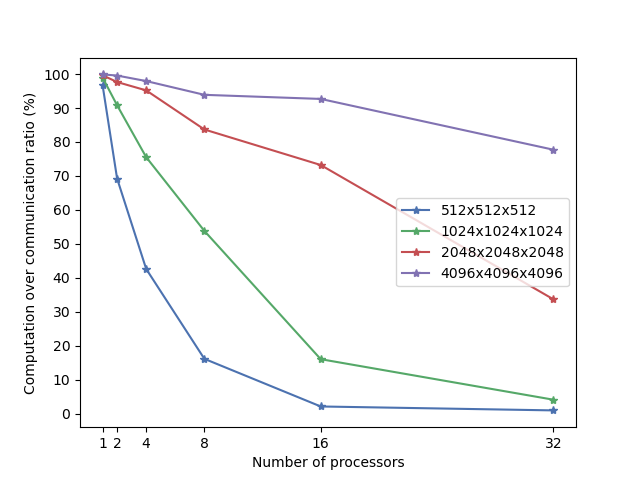
\includegraphics[width=0.8\linewidth]{figures/comp_over_comm.png}
    \caption{Computation over communication ratio on $P$ processors for the parallel algorithm, computed as $T_{\text{comp}}^p/T_{\text{total}}^p.$}
    \label{fig:compcomm}
\end{figure}

Considering also Figure \ref{fig:compcomm}, we can observe that for small matrices and high number of processors, the computation over communication ratio is particularly low, indicating that most of the time is spent on broadcasting $\textbf{B}$, scattering $\textbf{A}$ and gathering $\textbf{C}$ over actually computing the value of $\textbf{C}$; obviously this is an indication of "over-parallelization", reinforcing the well-known fact that the number of processors used should be adjusted to the size of the problem (as well as adapted to the specifics of the system used, since each network topology may be more or less susceptible to higher degrees of parallelization).
On a side note, Figure \ref{fig:compcomm} also shows the fact that the more processors we have, the higher the percentage of time spent on communicating gets for any size.

Additionally, figures like Figure \ref{fig:time_size} allow us to get an idea on the ideal number of processors to assign based on the sizes of the matrices; as mentioned earlier, a throughout analysis on the computation time is complex since it depends on both the network topology and the system load, and thus we need to rely on empirical observations to select the ideal number of processors for matrix multiplications of specific sizes.

\subsection{Speed up and scalability}

An interesting metric to consider is also the speed-up $S(P)$ provided by the parallelization process, computed as $S(P) = T_{\text{seq}}/T_{\text{parallel}}(P)$.

\begin{figure}[ht!]
    \centering
    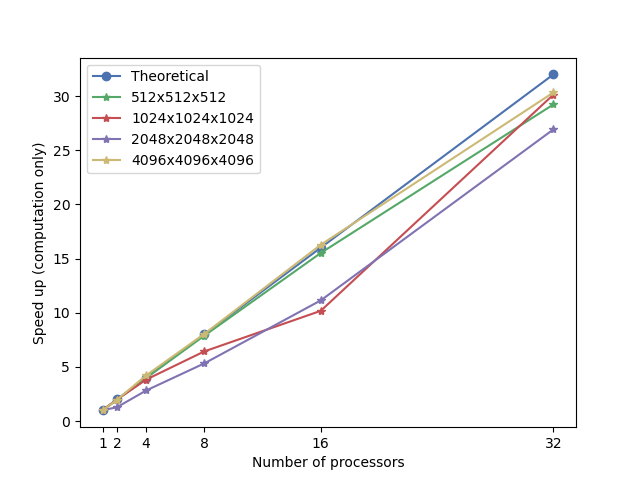
\includegraphics[width=0.8\linewidth]{figures/speedup_comp.png}
    \caption{Speed-up of parallel computation over sequential computation, computed as $S(P) = T_{\text{seq}}/T_{\text{comp}}(P)$. The theoretical speed-up refers to the speed-up theoretically obtainable by assuming the communication time to be negligible.}
    \label{fig:speedup_comp}
\end{figure}

As we mentioned in Section \ref{ssec:pperform}, the theoretical speed-up on the computation-only time provided by the parallelized algorithm is expected to be $S(P) = \Theta(P)$, and indeed Figure \ref{fig:speedup_comp} proves this bound.

\begin{figure}[hb!]
    \centering
    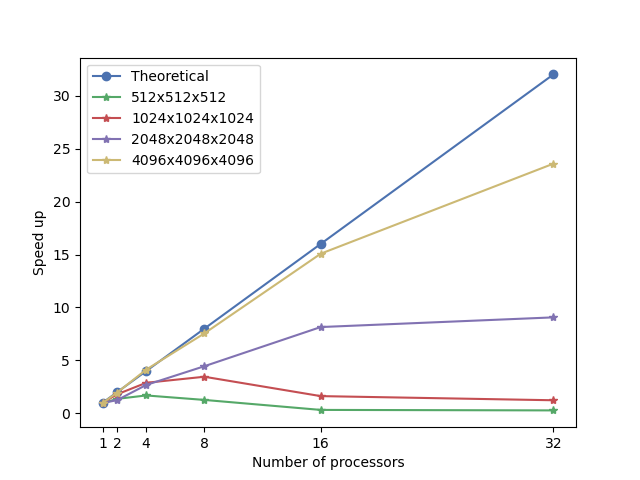
\includegraphics[width=0.8\linewidth]{figures/speedup.png}
    \caption{Speed-up of parallel algorithm over sequential one, computed as $S(P) = T_{\text{seq}}/T_{\text{parallel}}(P)$. The theoretical speed-up refers to the speed-up theoretically obtainable by assuming the communication time to be negligible.}
    \label{fig:speedup}
\end{figure}

However, the situation becomes again more complex as soon as we also factor in the communication time: Figure \ref{fig:speedup} shows the speed-up computed on $T_{\text{parallel}}(P)$ and highlights again how an excessive number of processors assigned overshadows the computation speed-up by an excessively dominating communication time. In particular, we can observe how the bigger the matrices are and the closer we are to the theoretical speed-up as the number of processor increases; additionally, we can also appreciate the fall-off caused by an over-increasing number of processors on smaller sizes of matrices.

Essentially, it is straightforward to see that on the CAPRI infrastructure our parallel algorithm is not scalable, since our experiments show how the speed-up factor decreases as the number of processors increases too much, even going into values lower than 1 (i.e. negative performance impact compared to the sequential algorithm) for the smaller matrices.
On a final note, it is worth to point out that, theoretically speaking, other network topologies may be able to scale better, but in practice such systems would be unfeasible and thus a certain degree of performance deterioration is likely to always be observed as the number of processors increases too much over the sizes of the matrices.
\section{Conclusions}

This project allowed us to take on the task of developing a parallel algorithm to make more efficient the execution of a real-world common problem like matrix multiplication, as well as the non-trivial task of developing measures to analyse the results of our parallelization approach.

In line with our expectation, we observed that a problem like matrix multiplication, which has an intrinsically high degree of parallelism, can achieve an ideal speed-up factor in parallel computation-only time over the sequential approach; however, as expected, the communication among processes required to enable the parallelization of the computation makes the whole algorithm not scalable indefinitely, thus the number of processors assigned should be considered carefully and, in particular, empirically, since in this very practical scenario a throughout analysis of the communication requirements is not possible.

\printbibliography[heading=bibintoc]

\end{document}
